\section{Zielsetzung}
\label{sec:ziel}
In diesem Versuch soll das Emissionsspektrum einer Kuperröntgenröhre aufgenommen und verschiedne Absorptionssprektren untersucht werden.

\section{Theorie}
\label{sec:Theorie}
In einer evakuierten Röhre werden mithilfe des \textit{glühelektrischen Effekts} Elektronen emittiert und auf eine Anode beschleunigt, wo sie beim Auftreffen
auf das Anodenmaterial Röntgenstrahlen emittieren. Bei dem Spektrum der entstehenden Röntgenstrahlen wird zwischen zwei verschiedenen Teilaspekten unterschieden, die zusammen
das in \autoref{fig:emissionsspektrum} abgebildete Spektrum ergeben.
\begin{figure}[H]
    \centering
    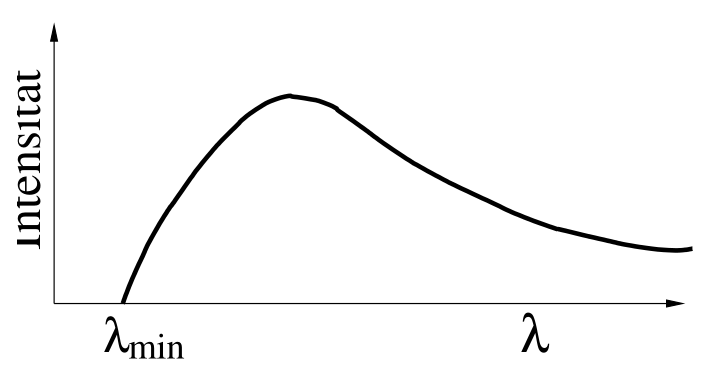
\includegraphics[width = 0.7 \textwidth]{data/emissionsspektrum.png}
    \caption{Schematische Darstellung des Emissionsspektrums einer Röntgenröhre \cite{Anleitung602}.}
    \label{fig:emissionsspektrum}
\end{figure}
\begin{enumerate}
    \item Das \textit{kontinuierliche Bremsspektrum} entsteht beim Abbremsen eines Elektrons im Coulombfeldes des Atomkerns, wobei ein Röntgenquant ausgesendet wird. Die Energie des Photons
    ist davon abhängig wieviel kinetische Energie des Elektrons abgegeben wird. Das Elektron muss dabei nicht nicht vollständig die Energie übertragen, weshalb das Spektrum kontinuierlich ist.
    Die minimale Wellenlänge, die übergeben werden kann ergibt sich zu,
    \begin{align}
        \label{eqn:wellenlaenge}
        \lambda_{\text{min}} = \frac{h\cdot c}{e_0 U}.
    \end{align}
    \item Das charakteristische Spektrum ernsteht dadurch, dass das Anodenamterial durch das Elekron ioniesiert wird. Es entsteht infolge des Ionisationsprozesses eine Leerstelle in einer inneren
    des Atomes, weshalb ein Elektron aus einer äußeren Schale unter Aussendung eines Röntgenquants auf die innere Schale zurückfällt. Die Energie des Röntgenquants ergibt sich aus der Energiedifferenz
    der beiden Energieniveaus,
    \begin{align}
        \label{eqn:energiedifferenz}
        h \nu = E_m - E_n.
    \end{align}
    Das charakteristische Spektrum besteht aus scharfen Linien, deren Energie charakteristisch für das Anodenmaterial der Röntgenröhre ist. Die Linien werden mit Buchstaben der Schale bezeichnet, auf der die Übergänge
    enden. Ein griechischer Buchstabe gibt an, von welcher Schale das Elektron ursprünglich kommt. Es ergibt sich somit zum Beispiel die $K_\alpha$-Linie, wobei ein Elektron aus der obersten Schale auf die K-Schale fällt.
\end{enumerate}
Durch die verschiedenen Elektronenhüllen wird das Coulombfeld des Kernes herabgesetzt, sodass die Bindungsenergie $E_n$ eines Elektrons auf der $n$-ten Schale folgt zu,
\begin{align}
    \label{eqn:verrEnergie}
    E_n = -R_\infty\cdot z_{\text{eff}}^2\cdot \frac{1}{n^2}.
\end{align}
Dabei steht $R_\infty$ für die Rydbergenergie und $z_{\text{eff}}$ für dei \textit{effektive Kernldadung} mit $z_{\text{eff}} = z - \sigma$, wobei $\sigma$ die Abschirmkonstante ist.
Die Abschirmkonstante unterscheidet sich für jedes Elektron und ist empirisch bestimmbar. So ergibt sich aus \eqref{eqn:verrEnergie} für die Energie $E_{K_\alpha}$ der $K_\alpha$-Linie 
der folgende Ausdruck
\begin{align}
    E_{K_\alpha} = R_\infty (z-\sigma_1)^2\cdot \frac{1}{1^2} - R_\infty (z-\sigma_2)^2 \cdot \frac{1}{2^2}.
\end{align}
Aufgrund des Bahndrehimpules und des Spins haben die äußeren Elektronen jedoch nicht alle dieselbe Bindungsenergie und somit haben die charakteristischen Linien eine Reihe von eng
aneinander liegenden Linien, die sogenannte \textit{Feinstruktur}. Im vorliegenden Versuch können jedoch nur die $K_\alpha$- und die $K_\beta$ Linien beobachtet werden, die die Bremsstrahlung überlagern. \newline

Bei einer Absorption von $\SI{1}{\mega\eV}$ Röntgenstrahlung sind der Compton- und der Photoeffekt die dominierenden Prozesse. Bei zunehmender Energie nimmt
der Absorptionskoeffizient immer mehr ab und steigt dann sprunghaft an, wenn die Photonenenergie gerade größer ist, als die Bundungsenergie eines Elektrons aus der nächsten Schale. Diese
\textit{Absorptionskanten} sind lageidentisch mit der Bindungsenergie des Elekrons $h\nu_{\text{abs}} = E_n - E_\infty$. Die Kanten werden analog zu den Absorptionslinien nach der Schale benannt aus der das Elektron stammt, $K$-. $L$-, $M$-, $\dots$, \textit{Absorptionskonstante}.
In \autoref{fig:absorptionsverlauf} ist eine schematische Darstellung des Absorptionsverlaufes bei zunehmender Energie abgebildet.
\begin{figure}[H]
    \centering
    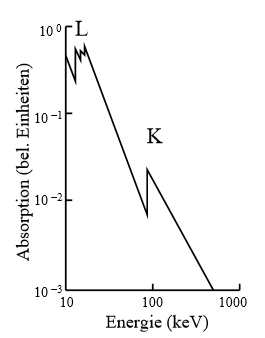
\includegraphics[width = 0.4 \textwidth]{data/absorptionsspektrum.png}
    \caption{Schematische Darstellung des Absorptionsverlaufes einer Röntgenröhre \cite{Anleitung602}.}
    \label{fig:absorptionsverlauf}
\end{figure}

Die Abschirmkonstante berechnet sich im folgenden Versuch für die $L$-Kanten mit der Energiedifferenz $\upDelta E_ = E_{L, \RN{2}} - E_{L, \RN{3}}$ nach dem folgenden Ausdruck,
\begin{align}
    \label{eqn:abschirmkonstante}
    \sigma_L = Z-\left(\frac 4\alpha \sqrt{\frac{\upDelta E_L}{R_\infty}} - \frac{5\upDelta E_L}{R_\infty}\right)^{\sfrac 12} \left(1+ \frac{19}{32}\alpha^2\frac{\upDelta E_L}{R_\infty}\right)^{\sfrac 12}.
\end{align}

Mithilfe der \textit{Brgg'schen Reflexion} kann die $n$-te Wellenlänge $\lambda$ durch die Gitterkonstante $d$ und dem Winkel $\vartheta$ durch 
\begin{align}
    \label{eqn:bragg}
    2d\sin(\vartheta)=n\lambda
\end{align}
bestimmt werden. Diese Gleichung kann dazu genutzt werden die Wellenlänge der Röntgenstrahlung zu bestimmen. Hier fallen Röntgenphotonen auf ein dreidimensionales Gitter und werden an jedem Atom des
Gitters gebeugt, wodurch die Röntgenstrahlen miteinander interferieren und unter dem Winkel $\vartheta$, dem \textit{Glanzwinkel}, konstruktive Interferenz erzeugen.